\subsection{Metodología}

Acorde con nuestro proyecto de trabajo terminal el cual implica el uso de diversas tecnologías, servicios en la nube y
el desarrollo de módulos interdependientes, se ha decidido adoptar la metodología ágil Scrum. La naturaleza del
proyecto, demanda un marco de trabajo flexible que permita adaptarse a las necesidades emergentes. Scrum, conocido
por su ligereza y adaptabilidad, es ideal para equipos pequeños y proyectos que buscan entregar valor de forma
incremental. Permite gestionar la complejidad y fomentar la colaboración, asegurando que las soluciones evolucionen
con el proyecto \cite{sutherland2020scrum}.

El desarrollo de la metodología Scrum se descompone en los siguientes pasos:


\begin{comment}
\begin{enumerate}
\setlength{\itemsep}{0pt}
    \item Reunión inicial de Stakeholders para generar una visión general del proyecto.
    \item El Product Owner define el \textit{Product Backlog}, que contiene los requerimientos del proyecto en forma de historias de usuario.
    \item Cada sprint inicia con una reunión de planificación, en la cual se seleccionan las historias de usuario prioritarias para incluir en el sprint.
    \item Se crea el Sprint Backlog, que contiene las tareas e historias de usuario a desarrollar durante el sprint.
    \item Durante la ejecución, se realizan Daily Standups breves, donde el equipo revisa avances y obstáculos.
    \item Al finalizar cada sprint, se efectúa una Sprint Review para presentar los avances al Product Owner.
    \item El Product Owner valida y acepta los entregables en caso de cumplir con los criterios definidos.
    \item Finalmente, se realiza una Sprint Retrospective para reflexionar sobre oportunidades de mejora.
    \item El ciclo se repite desde el paso 3 hasta concluir el proyecto.
\end{enumerate}
\end{comment}

\begin{enumerate}
\setlength{\itemsep}{0pt}
    \item Reunión inicial de Stakeholders para definir la visión del proyecto.
    \item El Product Owner define el \textit{Product Backlog} con los requerimientos en forma de casos de uso.
    \item Cada sprint inicia con una reunión de planificación para seleccionar los casos de uso prioritarios.
    \item Se crea el Sprint Backlog con las tareas a desarrollar durante el sprint.
    \item Durante la ejecución se realizan Daily Standups para revisar avances y obstáculos.
    \item Al finalizar cada sprint, se efectúa una Sprint Review para presentar avances al Product Owner.
    \item El Product Owner valida y acepta los entregables según los criterios definidos.
    \item Se realiza una Sprint Retrospective para identificar oportunidades de mejora.
    \item El ciclo se repite desde el paso 3 hasta concluir el proyecto.
\end{enumerate}

Para nuestro trabajo terminal, se plantean 5 sprints a lo largo de las dos fases del trabajo terminal:

\begin{enumerate}
    \item Trabajo Terminal I
    \begin{enumerate}
        \item Primer sprint. Se asignarán las tareas iniciales para definir y ajustar el alcance del proyecto. El primer paso será un análisis comparativo de los bosques de la Ciudad de México con el objetivo de seleccionar el más adecuado para el estudio. A continuación, se realizará la recolección manual de fotografías y una clasificación preliminar para crear el dataset de entrenamiento. Simultáneamente, se establecerá el entorno de trabajo y se avanzará en el diseño de la arquitectura híbrida. El resultado de este sprint será un dataset de imágenes en bruto, el diseño preliminar de la arquitectura híbrida y la documentación básica del proyecto.
        \item Segundo sprint. Se llevará a cabo el análisis de los modelos de aprendizaje automático y la preparación de la arquitectura híbrida. Se organizará el dataset recolectado con una estructura más clara, dejándolo listo para su uso. También se considerarán aspectos clave como la portabilidad y el despliegue, y se planificarán las interfaces de usuario para la aplicación móvil.
    \end{enumerate}
    \item Trabajo Terminal II
    \begin{enumerate}
        \item Tercer sprint. El enfoque principal será la limpieza y preparación final del dataset. Se procesarán las imágenes para normalizarlas y dividirlas en los subconjuntos necesarios. Con los datos listos, se iniciará el entrenamiento del modelo, se harán pruebas iniciales y se comenzará la optimización para mejorar la precisión y el rendimiento. De forma simultánea, se iniciará el desarrollo del backend del sistema.
        \item Cuarto sprint. Este sprint se centrará en la integración y consumo de la aplicación móvil. Se ajustarán los módulos restantes del sistema para asegurar una comunicación fluida y un funcionamiento coherente entre todas las partes de la solución. Se realizará el despliegue completo y la validación final del sistema con nuevas imágenes de prueba. Finalmente, se consolidará y completará la documentación del proyecto, resumiendo la metodología, la arquitectura, los resultados y las conclusiones.
    \end{enumerate}

\begin{figure}[H]
    \centering
     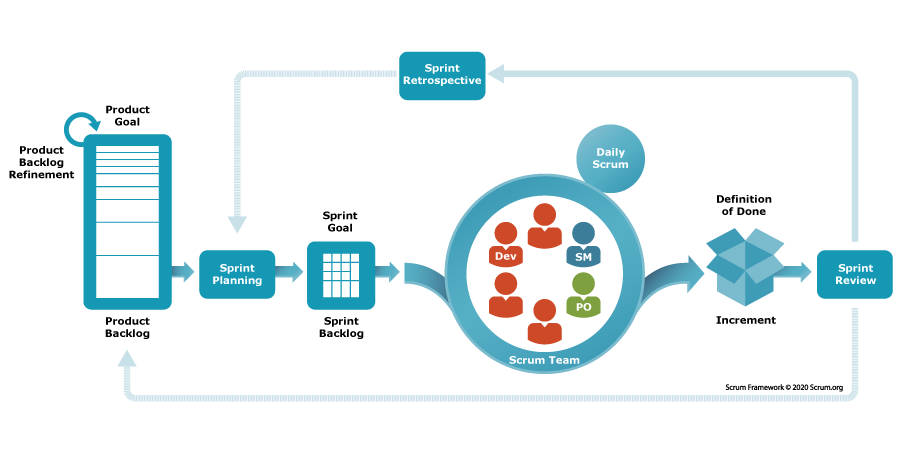
\includegraphics[width=1\textwidth]{images/C1/SCRUM.png}
    \caption{Metodología SCRUM. Tomado de \cite{scrumorg_que_es_scrum}}
    \label{fig:SCRUM}
\end{figure}

\end{enumerate}